\documentclass[a4paper]{article}

\usepackage[a4paper,  margin=1.0in]{geometry}

\usepackage{graphicx}
\usepackage{float}
\usepackage{hyperref}


\usepackage[utf8]{inputenc}
\begin{document}


\title{SNR classes project - birds species recognition using deep neural networks}

\author{Michał Sypetkowski, Marcin Lew, Filip Smurawa}
\maketitle

\section{General information}
Git repository \url{https://github.com/msypetkowski/SNR-proj.git}.
We use the following tools:
\begin{itemize}
    \item \textbf{Python}\footnote{\url{https://www.python.org/}}
    \item \textbf{OpenCV}\footnote{\url{https://opencv.org/}}
    \item \textbf{NumPy}\footnote{\url{http://www.numpy.org/}}
    \item \textbf{TensorFlow}\footnote{\url{https://www.tensorflow.org/ }}
\end{itemize}
We also use Tensorboard for model and training progress visualization.
The project is tested to run in Linux environment.

\section{Multilayer Perceptron}

\subsection{Data}
The data set consist of 50 subsets -- types of bird species.
Each subset is a set of 60 different pictures.
Altogether it gives us a data set of 3000 pictures.

We divided this dataset with ratio 0.1 (for testset)
so that the number of examples of each class is equal in both training and test set.
As a result we got 300 examples for test set and 2700 raw examples for training set.
Additionally, training set is augmented during training (see section \ref{augmentation}).


\subsection{Data augmentation}
\label{augmentation}
Every training image is randomly rotated, flopped or cropped. 
Augmented examples for example shown on figure \ref{fig:aug1}
are shown on figure \ref{fig:aug2}.

\begin{figure}[h]
    \caption[]{Not augmented example}
    \centering
    \includegraphics[page=2,width=0.1\textwidth]{aug1.png}
    \label{fig:aug1}
\end{figure}

\begin{figure}[h]
    \caption[]{Augmented examples}
    \centering
    \includegraphics[page=2,width=1.0\textwidth]{aug2.png}
    \label{fig:aug2}
\end{figure}


\subsection{HOG features}
We resize each image to 128x64x3 and we use
standard HOG features calculation procedure
(vectors of length 3780 are produced in this process).
We directly feed these vectors into our network.

\subsection{Model architecture}
We selected the architecture by experimenting.
Our network has 3 dense hidden dense layers of sizes 256, 128 and 64
Each of these layers have corresponding batch normalization layer.
After the last layer there is a softmax function.
We use cross enthropy as a loss function.
We tested 2 models with different activation functions:
\begin{itemize}
    \item relu
    \item sigmoid
\end{itemize}
Visualization of the model is shown on figure \ref{fig:arch}.

\begin{figure}[h]
    \caption[]{Tensorboard visualization of multilayer perceptron architecture (relu activation variant)}
    \centering
    \includegraphics[page=2,width=1.0\textwidth]{architecture.png}
    \label{fig:arch}
\end{figure}

\subsection{Results}
Accuracy and loss curves on training and validation set are shown on figure \ref{fig:training}.
Full results on testset for the model using relu are shown on figure \ref{fig:eval}.
Final accuracy of relu model is TODO and for sigmoid -- Y TODO.

\begin{figure}[h]
    \caption[]{Results on testset (blue - good answers)}
    \centering
    \includegraphics[page=2,width=1.0\textwidth]{eval.png}
    \label{fig:eval}
\end{figure}

% \begin{figure}[h]
%     \caption[]{Accuracy and loss curves}
%     \centering
%     \includegraphics[page=2,width=1.0\textwidth]{training.png}
%     \label{fig:training}
% \end{figure}

\section{Convolutional neural networks}
Not done yet.

\section{SVM}
Not done yet.



\end{document}
